% !BIB TS-program = biber
% FRL manuscript — single anonymized (authors on manuscript)
% Guide: main text <= 2500 words (excludes abstract, refs, tables, figures, captions, declarations)
% Flat files for EM: manuscript.tex, refs.bib, manuscript.bbl, Figure_1.png, highlights.txt
\documentclass[11pt,a4paper]{article}
\usepackage[margin=2.2cm]{geometry}
\usepackage{amsmath,amssymb}
\usepackage{booktabs}
\usepackage{graphicx}
\usepackage{setspace}
\usepackage[backend=biber,style=authoryear,maxcitenames=2,maxbibnames=99,uniquelist=false,giveninits=true]{biblatex}
\addbibresource{refs.bib}
\usepackage{xcolor}
\definecolor{darkblue}{rgb}{0.0,0.0,0.55}
\usepackage{hyperref}
\hypersetup{
  colorlinks=false,
  pdfborderstyle={/S/U/W 1},
  urlbordercolor=darkblue,
  linkbordercolor=darkblue,
  citebordercolor=darkblue,
}
\renewcommand{\UrlFont}{\ttfamily\color{darkblue}}
\onehalfspacing
\setlength{\parskip}{0.35em}
\setlength{\parindent}{1.2em}

\title{Does a Cointegration Filter Help in Forex Pairs Trading?}
\author{%
Tetiana Lemishko\textsuperscript{a,*}%
\quad
Alexandre Landi\textsuperscript{b,*}%
\quad
Juliana Caicedo-Llano\textsuperscript{c,d}\\[0.6em]
{\normalsize
\textsuperscript{a}Balanced Research, France
(affiliation at the time of writing)\\
\textsuperscript{b}SKEMA Business School, France\\
\textsuperscript{c}University of \'Evry Paris-Saclay, France\\
\textsuperscript{d}Regent's University London, United Kingdom}\\[0.4em]
{\small\textsuperscript{*}These authors contributed equally to this work (co-first authors).}\\[0.35em]
{\normalsize
Correspondence: Alexandre Landi,
\href{mailto:alexandre1.landi@skema.edu}{alexandre1.landi@skema.edu}}
}
\date{November 2026}

\begin{document}
\maketitle

\begin{abstract}
We ask whether an Engle--Granger--style tradability filter improves risk-adjusted
foreign-exchange pairs trading relative to an always-trade rule. Using daily Yahoo Finance
spot prices for seven major USD crosses from 2007 to 2025, we form all 21 undirected pairs
and trade equal-notional spreads on rolling 257/21-day train/test windows. The filter rule
trades an out-of-sample block only when a training-window residual ADF filter passes; the
benchmark uses the same z-score rule without that gate. After a stylized 2\,bp round-trip
cost, the unlevered filter portfolio earns about 0.5\% annualized at the pre-committed
entry band $z^{\star}=\pm 1$ because capital is rarely deployed---the invested fraction is
about 8\% of pair-days---yet it delivers higher Sharpe and Sortino ratios than always-trade.
A paired circular block bootstrap finds a statistically significant Sharpe gap
($\Delta=+0.59$, $p=0.014$) and Sortino gap ($\Delta=+0.68$, $p=0.018$) at $\pm 1$;
raw-return gaps are insignificant, and wider bands keep the ranking in point estimates without
statistical separation. The $\pm 1$ risk-adjusted edge survives a cost grid from 0 to 5\,bp.
The letter transfers equity-style pairs-filter horse races to liquid G10 FX; it is not a new
cointegration estimator, and residual ADF passes are not claimed as size-correct
cointegration detections at 5\%.

\vspace{0.45em}
\noindent\textbf{Keywords:} Cointegration; Pairs trading; Forex; Mean reversion; Sharpe ratio

\noindent\textbf{JEL classification:} C58; F31; G11; G15
\end{abstract}

\section{Introduction}

Pairs trading exploits temporary divergences between related assets
\parencite{gatev2006,krauss2017}. Distance and correlation filters treat mean reversion as a
short-horizon regularity; cointegration reframes the problem by requiring a stationary linear
combination of non-stationary prices, so that deviations from equilibrium are statistically
constrained \parencite{engle1987,vidyamurthy2004}. Equity applications of cointegration and
related selection filters are well documented
\parencite{huck2015,rad2015,galenko2012,burgess2003}. Parallel evidence for major currencies
is thinner, even though G10 USD crosses share a common numeraire and are linked by trade,
capital flows, and parity relations that make long-run co-movement economically \emph{plausible}
\parencite{fama1984,rogoff1996,engelwest2005,dunis2011}. Purchasing-power parity implies that
related nominal rates are not free to wander independently forever, even when real exchange
rates mean-revert only slowly \parencite{rogoff1996}. Covered and uncovered interest-rate
parity connect spots, forwards, and interest differentials; even when uncovered interest parity
fails as a short-horizon forecast \parencite{fama1984}, exchange rates remain asset prices
tightly tied to macro fundamentals \parencite{engelwest2005}. Those links motivate
\emph{where} we look; they do not, by themselves, deliver a trading rule, and we do not
estimate PPP baskets or trade UIP residuals.

This letter runs a clean selection-method horse race in liquid FX. We compare (i)~a
\emph{simple} pairs strategy that always trades the equal-notional synthetic spread on every
out-of-sample block with (ii)~a \emph{filter} strategy that trades only when an
Engle--Granger--style tradability filter \parencite{engle1987,vidyamurthy2004} passes on the
preceding training window. The design is deliberately close to equity filter evaluations such
as \textcite{huck2015}: same entry logic with and without the gate, stylized costs, and
portfolio-level risk-adjusted metrics. Ranking and forecasting approaches to pair selection
\parencite{huck2009,huck2010} are complementary but outside our design. The contribution is
transnational applicability of the filter logic to G10 FX---a setting that \emph{Finance
Research Letters} explicitly welcomes---not a new econometric procedure and not a
single-country equity replication.

Our pre-committed headline design is $z^{\star}=\pm 1$ with a stylized round-trip cost
$\kappa=2$\,bp of pair notional. At that design the filter book improves Sharpe and Sortino
with formal portfolio-level inference, but the economic reading is a \emph{filter} result:
unlevered filter-book returns are small because occupancy is low. We do not claim large
investable alpha. We also do not interpret residual ADF passes as MacKinnon-sized
``cointegration detected at 5\%'' \parencite{mackinnon1994,mackinnon2010}; the residual cutoff
is a pre-committed tradability tuning parameter in the sense of \textcite{vidyamurthy2004}.
Open replication code and a frozen price panel accompany the letter.

\section{Design}

\subsection{Data and windows}

Daily closes for EUR, GBP, JPY, CHF, CAD, AUD, and NZD against USD come from Yahoo Finance
\parencite{yahoo2024}, 1~January~2007 to 31~December~2025 ($T=4944$ calendar observations in
the frozen panel). Quotes with USD as numerator are inverted so every series is XXXUSD.
Analysis uses log prices. Missing values are forward-filled within the download pipeline and
dates with any incomplete cross-section are dropped, so the seven series share a common
calendar. Prices are processed in rolling blocks: a training window of $n=257$ days (about one
year) followed by a testing window of $m=21$ days (about one month). After each test block,
windows advance by $m$ days so the next train ends where the previous test ended. Training
samples estimate the hedge and the spread moments used in the out-of-sample z-score; the
simple rule skips the cointegration gate but still uses those moments. The 257/21 split is
pre-committed rather than optimized in-sample; we do not search over alternative window
lengths in this letter.

\subsection{Tradability filter}

We gate trading with the Engle--Granger two-step procedure \parencite{engle1987}, used as a
\emph{tradability filter} rather than as a formal size-correct cointegration test. Johansen
methods can recover multiple relations in larger systems; for bivariate FX pairs we keep the
Engle--Granger blueprint for transparency.

\emph{Step 1.} Ordinary ADF tests on each observed log-price level (constant; AIC lag). Both
legs must fail to reject a unit root ($p>0.05$).

\emph{Step 2.} OLS long-run regression $y_t=\alpha+\beta x_t+\varepsilon_t$ with residual
$\hat\varepsilon_t=y_t-\hat\beta x_t-\hat\alpha$.

\emph{Step 3.} Ordinary ADF test on $\hat\varepsilon_t$. We pass the window when the residual
ADF $p$-value is at most $0.05$ and use $\hat\beta$ as the hedge ratio for the synthetic
spread. Because $\beta$ is estimated, that residual statistic does \emph{not} follow the
Dickey--Fuller distribution of Step~1: a size-correct Engle--Granger test would compare it
against MacKinnon cointegration critical values, which are stricter (about $-3.36$ versus
$-2.87$ at the conventional 5\% level for $N=2$ with a constant on our 257-day windows;
\parencite{mackinnon1994,mackinnon2010}). We deliberately keep the looser ordinary-ADF residual
cutoff as a pre-committed tuning parameter that controls how permissive the filter is. A pass
means the residual looks stationary enough, under this operational rule, to trade the spread
out of sample---not that cointegration was detected at 5\%.

Cointegration is a relation, not a directed trading object, so we work with
$C(7,2)=21$ unordered pairs. Legs are ordered alphabetically by ticker. The residual filter
can depend on which series is the regressand; as a fixed design choice we therefore run both
OLS orientations on each training window and, among those that clear the residual cutoff,
retain the orientation with the clearer residual ADF $t$-statistic (more negative), mapping
that hedge into the alphabetical spread. If neither orientation passes, the pair is flat for
the following test window.

\subsection{Trading rule, costs, and portfolio}

On each testing day the z-score of the spread is
$Z_t=(\hat\varepsilon_t-\mu)/\sigma$, where $\mu$ and $\sigma$ are the training mean and
standard deviation of $\hat\varepsilon_t=\log P^{(1)}_t-\beta\log P^{(2)}_t$. Enter a long
spread when $Z_t<-z^{\star}$ and a short spread when $Z_t>z^{\star}$, for
$z^{\star}\in\{1,2,3\}$. Signals are lagged two days. Pair PnL is equal-notional,
$R_t=s_t\bigl(r^{(1)}_t-r^{(2)}_t\bigr)$, not $\beta$-hedged. Flat days enter the Sharpe
denominator as zeros.

Let $s_t\in\{-1,0,1\}$ denote the lagged signal. We charge a round-trip cost of $\kappa$
basis points of pair notional on position changes,
$\mathrm{cost}_t=(\kappa/10^{4})\times|s_t-s_{t-1}|/2$, so that opening or closing costs
$\kappa/2$\,bp and a long--short flip costs a full $\kappa$\,bp. Net returns are gross minus
cost. We report $\kappa\in\{0,1,2,5\}$, with headline results at $\kappa=2$\,bp---a stylized
all-in haircut for liquid G10 spot, not a full bid--ask plus rollover model. Swap costs are
left as a caveat.

The simple rule trades every testing window for every unordered pair. The filter rule trades
a testing window only if the tradability filter passes on the preceding training window.
Pair returns are averaged across the 21 pairs to form an unlevered $1/21$ book. Occupancy is
the mean \emph{invested fraction}: the average across days of (number of pairs with a nonzero
lagged signal)$/21$. Active days are the share of calendar dates with at least one live pair.

The 21 pairs are not independent experiments: every leg is a USD cross, and many pairs share
a second currency. Pair-level Sharpes are therefore descriptive of the cross-section, not
twenty-one separate hypothesis tests. Primary evidence is the portfolio comparison of filter
versus always-trade. On those two daily series we test whether Sharpe and Sortino differences
are distinguishable from zero with a paired circular block bootstrap that resamples calendar
dates once and applies the same blocks to both books, preserving contemporaneous cross-book
correlation \parencite{ledoitwolf2008}. Block length equals the 21-day test window
($B=10{,}000$). We studentize the Sharpe difference with a Newey--West HAC standard error
\parencite{neweywest1987} (Bartlett; lag from the $4(T/100)^{2/9}$ rule) and report a
percentile interval for Sortino under the paper's downside definition (standard deviation of
strictly negative daily returns). A HAC delta-method Sharpe check
\parencite{jobsonkorkie1981,memmel2003} agrees with the bootstrap. Calmar ratios remain
descriptive: maximum drawdown is path-dependent. The threshold $\pm 1$ is the pre-committed
headline design; $\pm 2$ and $\pm 3$ are reported alongside it.

As an implementable companion, on each training block we estimate pair spread volatility and
size every live pair on the following test block to 3\% annualized train-window volatility,
using the same leverage factor on both books; the companion book is the sum of pair PnLs, not
$1/21$. The 3\% cap is an arbitrary choice. Cumulative-return figures separately rescale the
filter path so that ex-post daily volatilities match the simple path; those figures are
visual aids only.

\section{Results}

Table~\ref{tbl:main} reports the headline unlevered book at $z^{\star}=\pm 1$ after
$\kappa=2$\,bp. The filter strategy earns 0.49\% annualized at 0.89\% volatility (Sharpe
0.55; Sortino 0.63) versus $-0.17\%$ at 4.02\% volatility for always-trade (Sharpe $-0.04$;
Sortino $-0.05$). Occupancy explains the gap in scale: invested fraction is 8.2\% for the
filter versus 51.3\% for always-trade, so most of the $1/21$ book is cash on a typical day.
Active days are 68\% versus 95\%. Maximum drawdown is $-2.5\%$ versus $-15.9\%$. Frictionless
Sharpes at $\pm 1$ are 0.62 (filter) and 0.01 (simple).

The risk-adjusted improvement is statistically separable at this design:
$\Delta\mathrm{Sharpe}=+0.59$ ($p=0.014$; 95\% studentized CI $[+0.12,+1.07]$) and
$\Delta\mathrm{Sortino}=+0.68$ ($p=0.018$; 95\% percentile CI $[+0.12,+1.28]$). The
annualized mean-return gap is not significant ($p=0.33$). That split is the filter story:
the filter's edge shows up in the volatility denominator, not in a large return differential.

At $\pm 2$, filter versus simple Sharpes are 0.41 versus 0.06, with invested fractions
3.0\% versus 19.2\% and maximum drawdowns $-1.9\%$ versus $-12.5\%$. At $\pm 3$, Sharpes are
0.48 versus 0.10, invested fractions 0.95\% versus 5.7\%, and drawdowns $-0.86\%$ versus
$-9.3\%$. The Engle--Granger gate itself is on for about 18.5\% of pair-days at every
threshold; always-trade fills almost all out-of-sample blocks. Bootstrap
$\Delta\mathrm{Sharpe}$ $p$-values are 0.145 and 0.089 at $\pm 2$ and $\pm 3$, and
$\Delta\mathrm{Sortino}$ $p$-values are 0.270 and 0.332, so wider bands keep the ranking in
point estimates without conventional statistical separation. We therefore treat $\pm 1$ as the
inferential headline and wider bands as descriptive robustness, consistent with the
pre-committed design rather than a post-hoc threshold search.

Across $\kappa\in\{0,1,2,5\}$, $\Delta\mathrm{Sharpe}$ at $\pm 1$ stays between $+0.57$ and
$+0.61$ with $p\le 0.015$; $\Delta\mathrm{Sortino}$ stays between $+0.65$ and $+0.69$ with
$p\le 0.021$. At $\pm 1$, frictionless Sharpes are 0.62 (filter) and 0.01 (simple); at
5\,bp they are 0.45 and $-0.12$. Block lengths of 5, 21, and 63 days leave the $\pm 1$
conclusion unchanged, as does dropping the initial warm-up zeros before the first completed
train/test cycle.

\begin{table}[ht]
\centering
\caption{Unlevered $1/21$ portfolio at $z^{\star}=\pm 1$ after $\kappa=2$\,bp round-trip
costs (257/21 windows; 21 undirected pairs; 2007--2025). $\Delta$ rows are filter minus
always-trade from a paired circular block bootstrap ($B=10{,}000$; block length 21).
Occupancy is independent of $\kappa$.}
\label{tbl:main}
\begin{tabular}{lrr}
\toprule
Metric & Filter & Always-trade \\
\midrule
Ann.\ return (\%) & 0.49 & $-0.17$ \\
Ann.\ volatility (\%) & 0.89 & 4.02 \\
Sharpe & 0.55 & $-0.04$ \\
Sortino & 0.63 & $-0.05$ \\
Calmar & 0.20 & $-0.01$ \\
Max.\ drawdown (\%) & $-2.48$ & $-15.89$ \\
Invested fraction (\%) & 8.24 & 51.27 \\
Active days (\%) & 68.33 & 94.58 \\
$\Delta$Sharpe ($p$) & \multicolumn{2}{c}{$+0.59$ (0.014)} \\
$\Delta$Sortino ($p$) & \multicolumn{2}{c}{$+0.68$ (0.018)} \\
\bottomrule
\end{tabular}
\end{table}

Figure~\ref{fig:cum} shows equal ex-post volatility cumulative returns at $\pm 1$ after
$\kappa=2$\,bp. The filter path rises more steadily than the always-trade path, which
suffers deeper early-sample drawdowns. The figure is a visual aid only: the main claim is the
unlevered portfolio comparison in Table~\ref{tbl:main}.

\begin{figure}[ht]
\centering
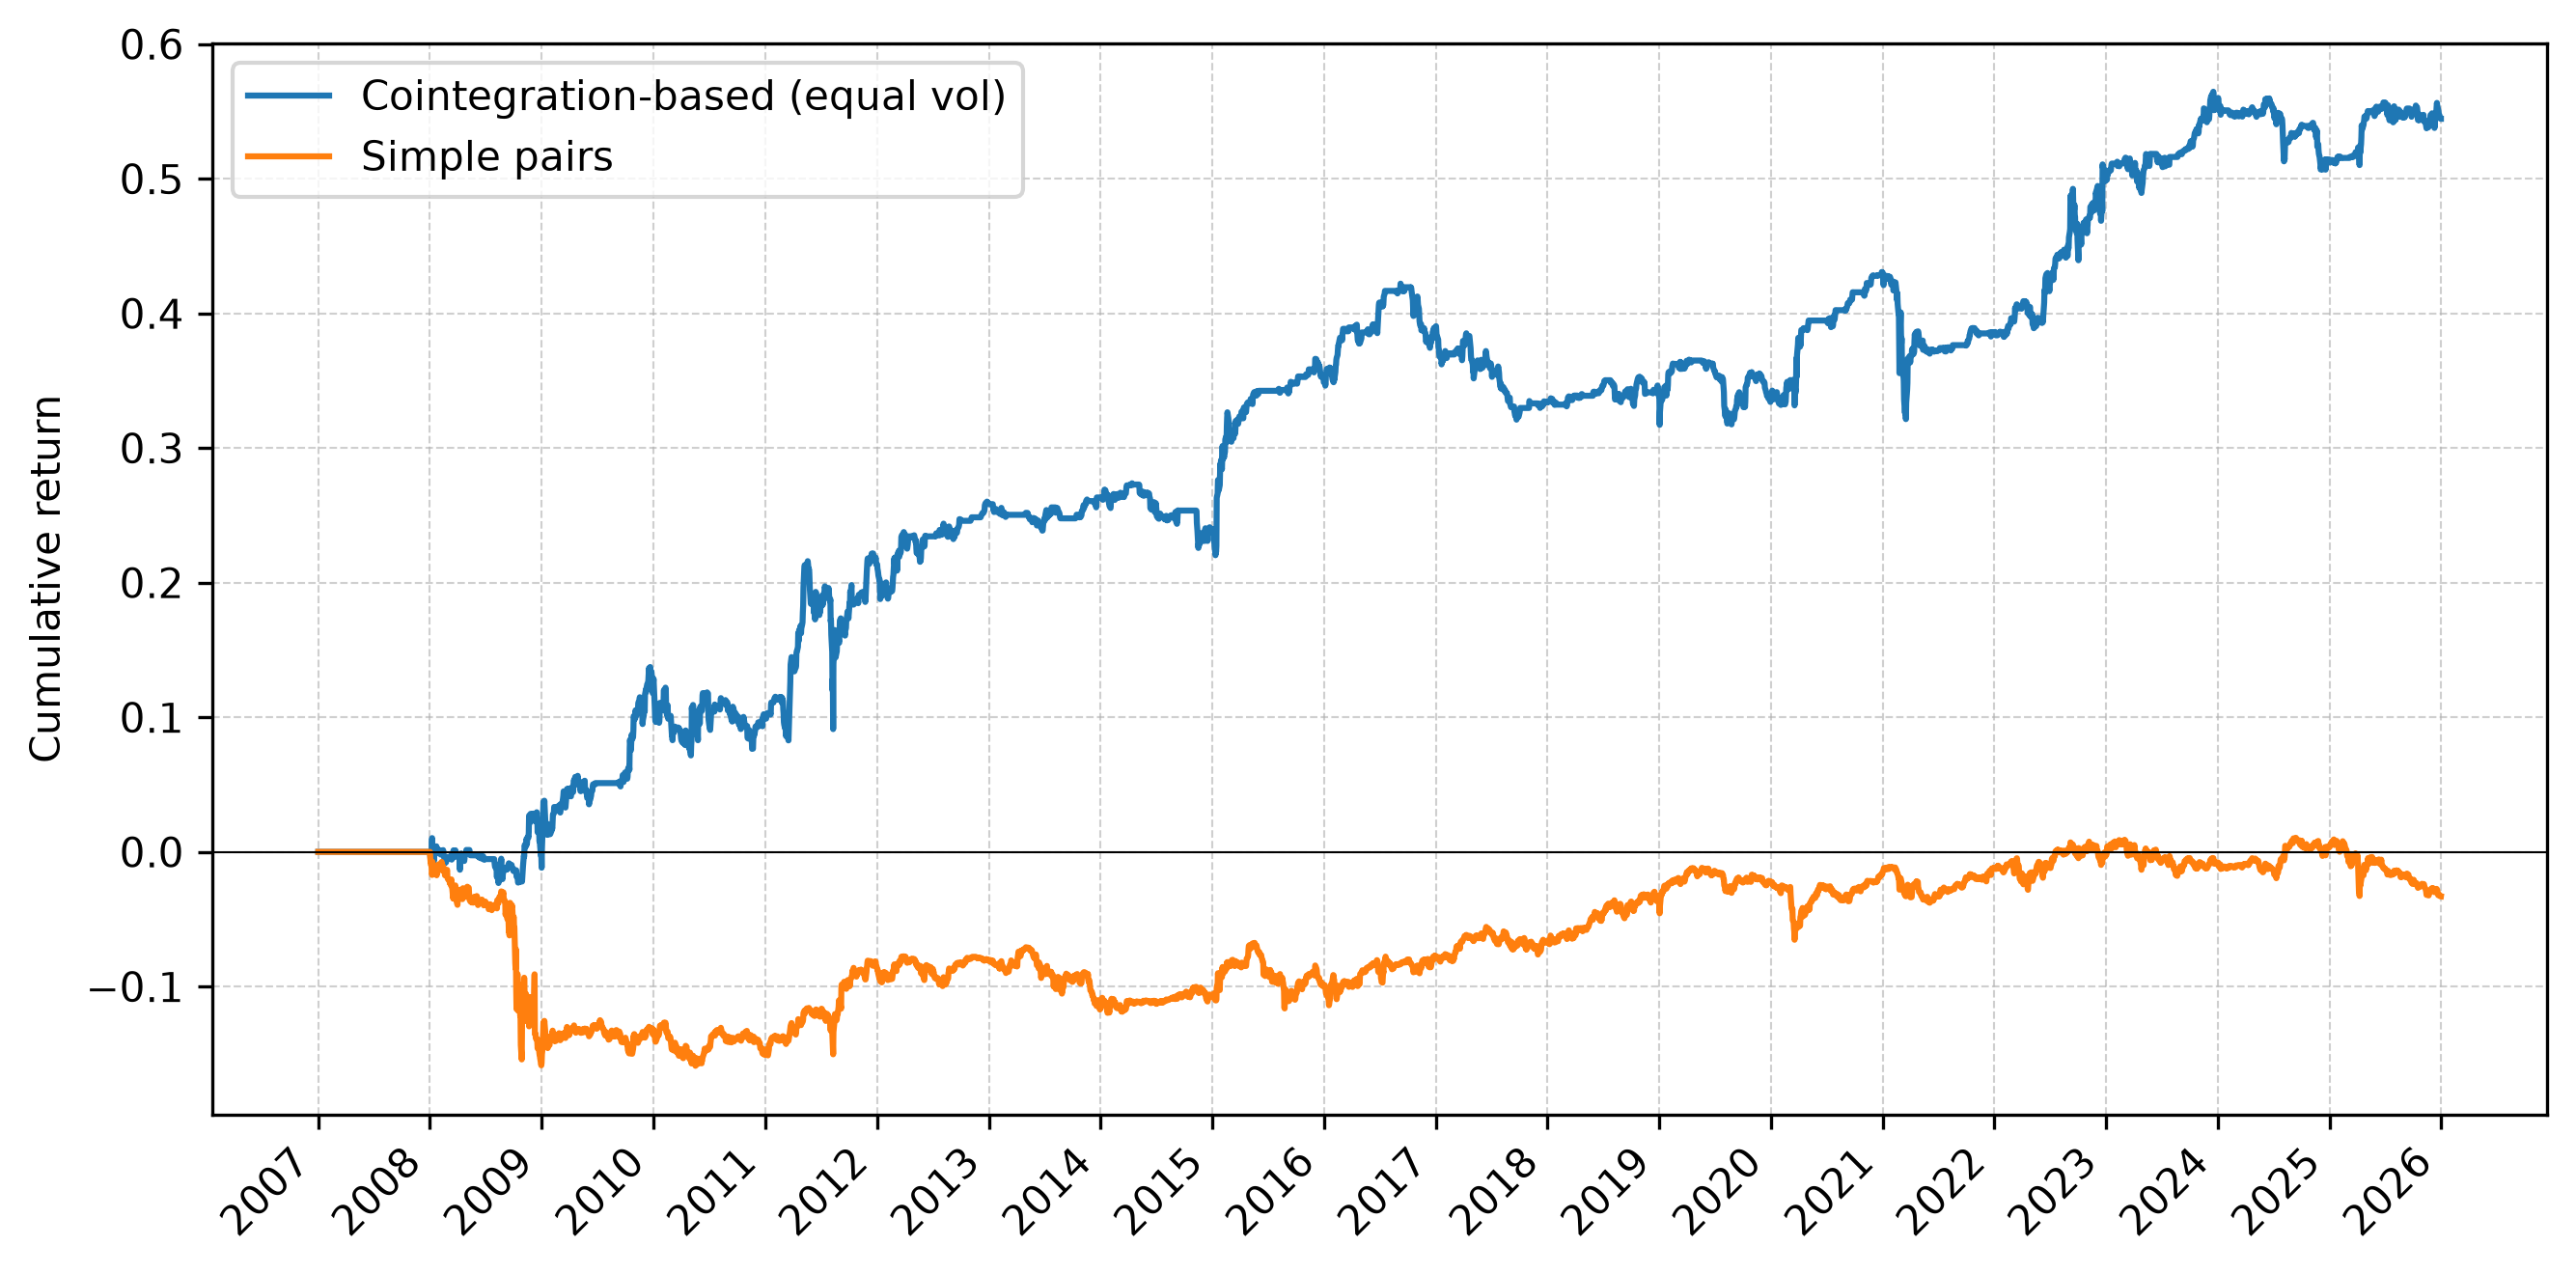
\includegraphics[width=0.92\textwidth]{Figure_1.png}
\caption{Cumulative returns at $z^{\star}=\pm 1$ after $\kappa=2$\,bp, with the filter
path scaled to equal ex-post daily volatility versus always-trade (visual comparison only).}
\label{fig:cum}
\end{figure}

Sizing each live pair to 3\% train-window volatility raises the filter companion to about
3.9\% annualized return at about 8.3\% book volatility (Sharpe 0.47) versus 1.9\% return at
22.0\% volatility for always-trade (Sharpe 0.09). Book volatility follows how many pairs are
live under a common per-pair rule; the companion does not force equal occupancy.

Two caveats keep the claim honest. First, Yahoo spots are a convenience sample; we treat the
exercise as a ranking horse race under a frozen public panel, not as executable prime-broker
PnL. Absolute return levels could move under a professional vendor, but the object of interest
is whether the filter ranks above always-trade after the same costs and the same portfolio
construction. Second, equal-notional PnL does not match the estimated hedge ratio used to form
the spread; $\beta$-hedged returns are left to companion work. Overnight swaps are outside the
stylized $\kappa$ grid; short test windows and frequent flats limit overnight exposure relative
to a always-on book, but they do not eliminate financing frictions. Flats mechanically compress
volatility, which is why invested fraction and active days belong beside Sharpe in the main
table: without occupancy, a reader can mistake a low-vol filter for a high-capacity strategy.
Replication materials (frozen parquet, \texttt{uv} pipeline, and bootstrap script) are linked
in the data-availability statement so that the $\Delta$Sharpe and $\Delta$Sortino tests can be
recomputed from the same panels.

\section{Conclusion}

In liquid G10 FX, gating an equal-notional pairs rule with an Engle--Granger--style
tradability filter improves Sharpe and Sortino at the pre-committed band $z^{\star}=\pm 1$
after stylized costs, with paired block-bootstrap support. Raw returns remain small because
the filter keeps occupancy low: about 8\% of pair-days are live at $\pm 1$, versus about
half the book under always-trade. Wider entry bands preserve the point-estimate ranking
without statistical separation. A 3\% per-live-pair volatility companion still ranks the
filter first on Sharpe, at higher book volatility that scales with how many pairs are on.
The letter transfers an equity-style pairs-filter evaluation to major FX; it does not propose
a new estimator, and the residual ADF cutoff is an operational tradability rule rather than a
MacKinnon-sized cointegration claim. Tightening that cutoff to formal Engle--Granger critical
values, aligning PnL with the estimated hedge, and adding parity-based or Johansen filters
are natural extensions for future work.

\section*{Funding}
This research did not receive any specific grant from funding agencies in the public,
commercial, or not-for-profit sectors.

\section*{Data availability}
Daily FX spots and replication scripts are available at
\url{https://github.com/QuantLandi/fx-cointegration} (frozen Yahoo-derived panel
\texttt{data/fx\_prices.parquet}; MIT code/data; CC~BY~4.0 manuscript assets under
\texttt{paper/}).

\section*{Declaration of competing interests}
The authors declare that they have no known competing financial interests or personal
relationships that could have appeared to influence the work reported in this paper.

\section*{CRediT authorship contribution statement}
\textbf{Tetiana Lemishko:} Conceptualization, Methodology, Investigation, Formal analysis,
Writing -- original draft, Writing -- review and editing.
\textbf{Alexandre Landi:} Conceptualization, Methodology, Software, Formal analysis, Data
curation, Visualization, Writing -- review and editing, Project administration.
\textbf{Juliana Caicedo-Llano:} Conceptualization, Supervision, Writing -- review and editing.

\printbibliography

\end{document}
